\section{Results}
\label{sec:results}

\subsection{The size of the surface}

Table~\ref{tab:corpus} summarises the corpus and the classification outcome per
registry. The headline is the mismatch between the two ways of counting. Hooks
appear in 8.4 percent of versions, which sounds containable, but those versions
absorb 31 percent of installs, because hook-bearing packages are build tooling
and build tooling is a transitive dependency of nearly everything. A policy
that treats hooks as a rare exception is reasoning from the wrong denominator.

\begin{table*}[t]
  \centering
  \footnotesize
  \caption{Corpus and classification by registry over 19 months. Install share
  is the fraction of total registry download volume attributable to versions
  that declare a hook. Malicious and reckless counts are distinct packages, not
  versions, after the manual review of Section~\ref{sec:methodology}.}
  \label{tab:corpus}
  \begin{tabular}{l rrr rr rrr}
    \toprule
    \multirow{2}{*}{Registry}
      & \multicolumn{3}{c}{Corpus}
      & \multicolumn{2}{c}{Hook prevalence}
      & \multicolumn{3}{c}{Classification (packages)} \\
    \cmidrule(lr){2-4} \cmidrule(lr){5-6} \cmidrule(lr){7-9}
      & Versions & With hook & Executions
      & \% versions & \% installs
      & Malicious & Reckless & Inconclusive \\
    \midrule
    A (JavaScript) & 812{,}400 & 79{,}910 & 3{,}944{,}200 & 9.8 & 38.1
                   & 31 & 124 & 902 \\
    B (Python)     & 431{,}700 & 30{,}260 & 1{,}612{,}800 & 7.0 & 24.6
                   & 12 &  49 & 411 \\
    C (Ruby)       & 178{,}100 &  9{,}230 &   549{,}400 & 5.2 & 19.8
                   &  4 &  17 & 143 \\
    \midrule
    Total          & 1{,}422{,}200 & 119{,}400 & 6{,}106{,}400 & 8.4 & 31.0
                   & 47 & 190 & 1{,}456 \\
    \bottomrule
  \end{tabular}
\end{table*}

\subsection{Behaviour separates}

The benign majority is strikingly uniform. A legitimate compilation hook
execs a compiler, writes into the package directory, reads system headers, and
exits. It does not open a socket. Across 119{,}400 hooks, only 2{,}214, or 1.9
percent, contacted a host outside the registry allowlist, and only 408 read
credential material outside the package tree.

Because the benign behaviour is so narrow, a single feature does most of the
work. Network contact alone recovers 94 percent of our confirmed malicious set
at a false positive rate of 1.8 percent against the manual review, and the
conjunction used in Algorithm~\ref{alg:classify} raises precision to 87 percent
while giving up 4 points of recall. Figure~\ref{fig:features} shows how the
three signals distribute across the labels.

\begin{figure}[t]
  \centering
  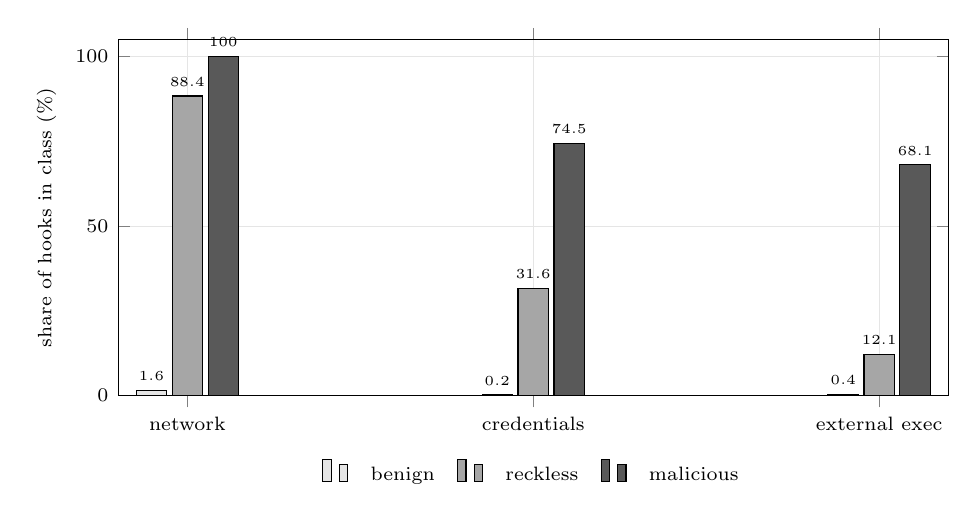
\begin{tikzpicture}
    \begin{axis}[
        width=\linewidth, height=6.1cm,
        ybar, bar width=11pt,
        ylabel={share of hooks in class (\%)},
        symbolic x coords={network, credentials, external exec},
        xtick=data,
        xticklabel style={font=\scriptsize},
        ymin=0, ymax=105,
        legend style={font=\scriptsize,at={(0.5,-0.16)},anchor=north,
                      draw=none,fill=none,legend columns=3,column sep=1.4ex},
        grid=major, grid style={gray!20},
        tick label style={font=\scriptsize},
        label style={font=\scriptsize},
        nodes near coords, nodes near coords style={font=\tiny},
      ]
      \addplot[fill=black!10,draw=black] coordinates {
        (network,1.6) (credentials,0.2) (external exec,0.4)
      };
      \addlegendentry{benign}
      \addplot[fill=black!35,draw=black] coordinates {
        (network,88.4) (credentials,31.6) (external exec,12.1)
      };
      \addlegendentry{reckless}
      \addplot[fill=black!65,draw=black] coordinates {
        (network,100.0) (credentials,74.5) (external exec,68.1)
      };
      \addlegendentry{malicious}
    \end{axis}
  \end{tikzpicture}
  \caption{Prevalence of each behavioural signal within each class. Benign
  hooks essentially never open a socket, which is why a single network feature
  is nearly sufficient for detection.}
  \label{fig:features}
\end{figure}

\subsection{A precursor the registries already have}

The most actionable result is not about hooks at all. For each malicious
package we reconstructed the maintainer account's public event history. Thirty
five of the 47 malicious versions were published within 72 hours of a change to
the account's recovery email address, and 29 within 24 hours. The base rate is
far lower: across all packages with a recovery-email change in the same period,
only 0.11 percent published any version within 72 hours, because a legitimate
maintainer who updates their email does not usually ship immediately
afterwards.

Registries hold this data. None of the three publishes a version during a
cooling-off window after an account recovery change, and none flags the
combination for review. A 72-hour hold on hook-bearing publications following
a recovery-email change would have delayed 35 of 47 malicious versions past the
median time to detection in our corpus, at a cost of delaying roughly 140
legitimate publications per month across the three registries.

\subsection{Time to withdrawal}

Malicious versions live longer than the incident reports suggest. Median time
from publication to withdrawal was 31 hours, and the ninetieth percentile was
9.4 days. Two packages remained available for the entire 19-month window and
were withdrawn only after our disclosure. Since a continuous integration runner
resolves fresh dependency versions on every build, a 31-hour window is many
thousands of installs for a package deep in a popular tree.
